% technologien.tex
\section{R, RStudio, Pakete}
\label{kapitel:R}
\begin{figure}[!t]
\centering
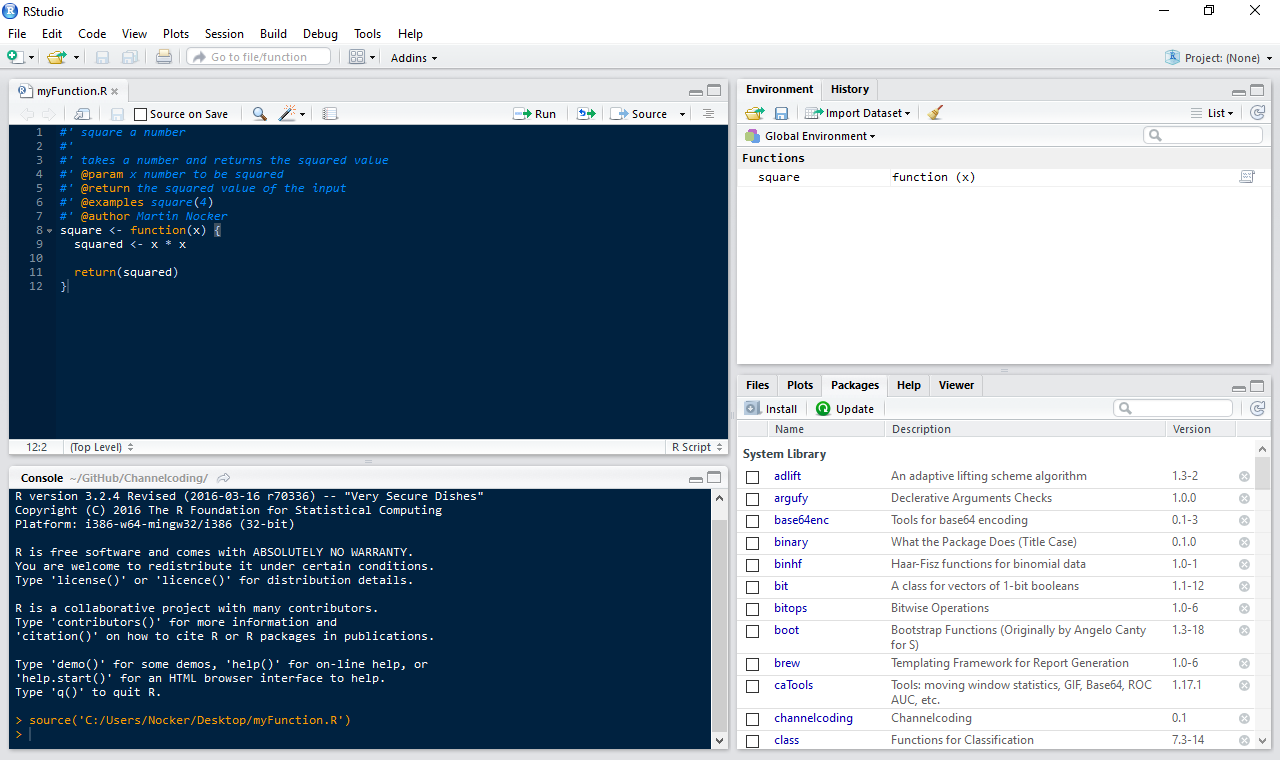
\includegraphics[width=\textwidth]{abbildungen/rstudio}
\caption{RStudio Standardansicht}
\label{abb:rstudio}
\end{figure}
% R
R ist eine, im Jahre 1992 entwickelte, schwach und dynamisch typisierte Programmiersprache, die vor allem in der Statistik für die Analyse von großen Datenmengen Anwendung findet. Ein weiteres Motiv für die Verwendung von R sind die vielseitigen Möglichkeiten, bei gleichzeitig einfacher Handhabung, graphischer Darstellungen großer Datenmengen. R-Code wird nicht kompiliert, sondern nur interpretiert und ist daher platformübergreifend verwendbar. Datentypen müssen zur Übersetzungszeit nicht bekannt sein. Die Typüberprüfung findet zur Laufzeit statt. Diese Eigenschaft erschwert das Finden von Fehlern im Code erheblich.
\\
\\
% R Pakete TODO! Cite
Der Funktionsumfang der Sprache kann durch sogenannte Pakete erweitert werden. Bei der Installation von R sind die wichtigsten Pakete inkludiert. Über Repositories wie CRAN\footnote{The Comprehensive R Archive Network: \url{https://cran.r-project.org/}} oder GitHub sind über 8000 zusätzliche Pakete (Stand: Mai 2016) für die verschiedensten Anwendungsbereiche verfügbar. Diese Vielfalt an Paketen ist ein Grund für den Erfolg von R [R Packages]. Pakete werden laufend aktualisiert und verbessert. Selbst entwickelte Pakete können via CRAN für andere Entwickler veröffentlicht werden, müssen jedoch strenge Auflagen zur Aufrechterhaltung der Konsistenz bei Inhalt, Form und Dokumentation der Pakete einhalten \cite{rmanual}.  
\\
\\
% Roxygen TODO! Lesen!
Ein wichtiges Paket welches im Rahmen dieser [Bachelor]arbeit verwendet wurde ist \emph{roxygen}. Mithilfe dieses Pakets wird, ähnlich wie JavaDoc für Java, durch spezielle Kommentare und Annotations überhalb der Paketfunktionen automatisch die Paketdokumentation erstellt. Die roxygen-Kommentare der Paketfunktionen, die für wartbaren Code ohnehin unabdingbar sind, sind für den Entwickler erheblich angenehmer als die Paketdokumentation von Hand zu schreiben. Roxygen-Kommentare werden durch das Kommentarsymbol #' am Zeilenbeginn eingeleitet. Zu den wichtigsten Annotations gehören jene für die Beschreibung der Parameter (@param) und Rückgabewerte (@return) sowie Beispiele zur Ausführung der Funktion (@examples). Weiters wird über die @export Annotation geregelt welche Funktionen nach Auslieferung des Pakets von außen aufrufbar sind.
\\
\\
% RStudio
RStudio ist eine freie und open source Entwicklungsumgebung für R. Abbildung \ref{abb:rstudio} zeigt die Version 0.99.893.
%% Daniel %%
Die weitverbreiteste Entwicklungsumgebung für die Programmiersprache R ist das RStudio, das in der Abbildung \ref{abb:rstudio} zu sehen ist. Diese Umgebung wurde speziell für den Softwareentwurf mittels R entwickelt und stellt alle wichtigen Funktionen zu Verfügung. Damit ist es besonders einfach selber R-Pakete zu entwickeln, oder andere Programmiersprachen mittels speziellen Schnittstellen mit R zu verbinden. Zur Visualisierung von den Berechnungsergebnissen sind bereits einige Vorlagen in die Entwicklungsumgebung integriert. Zum Beispiel ist es sehr einfach HTML Seiten, PDF Dokumente oder auch interaktive Oberflächen mittels \emph{Shiny} zu erstellen. Um dynamische Dokumente zu erstellen kann auch \emph{RMarkdown} verwendet werden, das wird im Kapitel \ref{kapitel:rmarkdown} näher erklärt.
\section{C++, Rcpp}
\label{kapitel:rcpp}
Manchmal ist R-Code einfach nicht schnell genug. Typische Flaschenhälse sind Schleifen und rekursive Funktionen. Die Performance kann in solchen Fällen durch Auslagern von Funktionen und Algorithmen in C oder C++ erheblich verbessert werden, da der Code kompiliert und somit optimiert werden kann anstatt nur interpretiert zu werden.\\
R bietet drei Möglichkeiten C/C++ Code aufzurufen:
\begin{itemize}
	\item \emph{.C} native Schnittstelle
	\item \emph{.Call} Schnittstelle
	\item \emph{Rcpp} Paket
\end{itemize}
%% Daniel %%
In manchen Situationen ist R nicht schnell genug für die spezielle Anwendung, deswegen kann man auf C oder C++ zurückgreifen. Vorallem die Geschwindigkeit bei Schleifen ist aufgrund der schwachen Typisierung in R relativ schlecht. Darum kann man bei einer intensiven Nutzung von Schleifen auf C oder C++ zurückgreifen und mit einer speziellen Schnittstelle diesen Code von R aufrufen.
\\
\\
Grundsätzlich gibt es 3 Möglichkeiten C/C++-Code von R aufzurufen:
\begin{itemize}
	\item \emph{.C} native Schnittstelle
	\item \emph{.Call} Schnittstelle
	\item \emph{Rcpp} Paket
\end{itemize}
\\
Die \emph{.C} Schnittstelle ist die einfachste Variante C Code auszuführen, jedoch auch jene mit den größten Einschränkungen. Im C Code sind keinerlei R Datentypen oder Funktionen bekannt. Alle Argumente sowie der Rückgabewert müssen als Zeiger in der Parameterliste übergeben werden deren Speicher vor dem Aufruf reserviert werden muss.
\\
\\
Bei der \emph{.Call} Schnittstelle handelt es sich um eine Erweiterung der \emph{.C} Schnittstelle. Die Implementierung ist komplexer, dafür sind R Datentypen verfügbar und es gibt die Möglichkeit eines Rückgabewerts mittels dem return Statements. \cite{wickham2015r}
\\
\\
Bei den ersten beiden Möglichkeiten muss der C Code vor dem Aufruf per Hand kompiliert und in der R Session geladen werden. Das \emph{Rcpp} Paket ermöglicht die Verwendung von C++ Code ohne diesen Aufwand. Im C++ Code stehen R Datentypen wie Vektoren, Matrizen oder Listen ohne kompliziertem Syntax zur Verfügung. Die Funktionsaufrufe sehen, im Gegensatz zu den ersten beiden Ausführungen, aus wie normale R Funktionsaufrufe und macht dadurch den Code erheblich lesbarer. Weiters stehen Vektorfunktionen zur Verfügung, d.h. eine auf einen Vektor angewandte Funktion wird auf jedes Vektorelement ausgeführt und erspart somit beispielsweise eine Schleife. Bei der Entwicklung eines eigenen Pakets ist es bei der Verwendung des \emph{Rcpp} Pakets zusammen mit RStudio sehr einfach C++ Code zu integrieren. Während der Paketerzeugung kompiliert RStudio automatisch alle C++ Dateien und erstellt automatisch Wrapper-Funktionen, die den Zugriff auf die Funktionen erleichtern. Die genaue Verwendung des \emph{Rcpp} Pakets ist in \cite{wickham2015advanced} beschrieben/ nachzulesen.
\section{RMarkdown, \LaTeX, Ti\textit{k}Z}
\label{kapitel:rmarkdown}
\begin{figure}[!t]
\centering
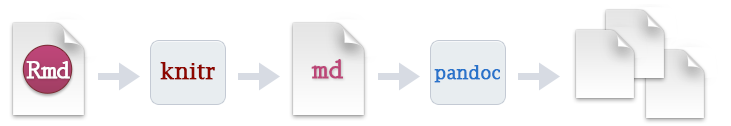
\includegraphics[width=\textwidth]{abbildungen/rmarkdown}
\caption{RMarkdown Überblick, Quelle: \cite{rmarkdown}}
\label{abb:rmarkdown}
\end{figure}
% R Markdown
Zur Erstellung von dynamischen Dokumenten kann das Paket \emph{RMarkdown} verwendet werden. Durch die Kombination der Syntax von Markdown, R, \LaTeX\ und HTML ergibt sich ein flexibles und einfaches Werkzeug. Die unterstützen Ausgabeformate beinhalten u.a. HTML, PDF, MS Word und Beamer (Präsentationen).
\\
\\
% R Markdown Workflow
Abbildung \ref{abb:rmarkdown} zeigt den Workflow für die Generierung eines dynamischen Dokuments mittels \emph{RMarkdown}. Der Markdown, R und \LaTeX\ Code wird zusammen mit dem gewünschten Ausgabeformat, wobei mehrere Angaben möglich sind, in die \emph{RMarkdown}-Datei (Dateiendung .rmd) geschrieben. Die RMD-Datei wird dem \emph{knitr} Paket übergeben, welches den R Code ausführt und eine neue Markdown-Datei (Dateiendung .md) erstellt, die den R Code und dessen Ergebnisse beinhaltet. Die erzeugte Markdown-Datei wird von \emph{pandoc} weiterverarbeitet, was für die Erstellung des endgültigen Dokuments im gewünschten Format zuständig ist. Bei der Verwendung von RStudio ist \emph{pandoc} automatisch verfügbar. Den eben beschriebenen Ablauf kapselt das \emph{RMarkdown}-Paket in einen einzigen \emph{render}-Funktionsaufruf.
\\
\\
% LaTeX, TikZ